\nopagebreak
\section{Energy Modelling}\label{sec:energy-models}

An energy model provides information on the energy consumed when running a program on a given hardware platform, based on parameters that characterise the program and its execution. The energy model contains measured energy consumption costs for these parameters and links these costs to program specific values for the parameters to arrive at an overall energy consumption estimation. 

Models that support software energy analysis typically associate program constructs, such as source code blocks, basic blocks in the intermediate representation of the program used during compilation or machine code instructions, with energy consumption costs. In addition, other costs arising from the execution of a program may need to be considered, depending on the micro architectural features of the hardware; examples are costs associated with the memory hierarchy, such as the cost of a cache hit and miss or the cost of accessing on-chip and off-chip memory, and also costs associated with the processor pipeline, such as the cost of pipeline stalls. In addition, the cost of the processor being idle and the cost of processing multiple threads concurrently may also need to be considered. 
%
In general, to instantiate an energy model, model parameters can be obtained either from analyzing execution or simulation traces, e.g.\ counting instructions, cache hits and misses, etc, or through static analysis as will be discussed next, in Section~\ref{sec:energy-analysis}.

The challenge in energy modelling for software energy analysis is in finding a good compromise between the accuracy of the model and the ease with which the information can be mapped onto software constructs. Regarding the former, model accuracy tends to be higher for models at the lower-levels of abstraction, i.e.\ instruction-level energy models are typically more accurate than energy models at the intermediate representation of the compiler, and source code energy models are less accurate in comparison. 
%
However, understanding which source code lines or blocks consume most energy is much more useful to software developers looking to optimise their code for energy efficiency, than knowing the energy consumed by the sequence of machine instructions issued by the compiler. The higher the level of abstraction at which the information is presented to the software developer, the easier it is for them to comprehend the impact of algorithms and coding on the energy consumed during program execution. Yet, taking measurements to characterize energy models is simplest and most accurate when performed at the lower levels of abstraction, where energy costs of low-level software constructs such as machine instructions can be determined directly.



\subsection{Defining and constructing an energy model at ISA level}

The Instruction Set Architecture (ISA) is the interface between hardware and
software. 
%
It defines the hardware architecture and its behaviour in terms of low-level
programming constructs such as supported data types, machine instructions,
registers, the memory architecture, any interrupt and exception handling as
well as I/O operations.
%
The ISA provides a practical level of abstraction for energy modelling, because
it is possible to directly correlate the energy consumption of the hardware
operations associated with instruction execution to low-level software
constructs.

Energy modelling at ISA level dates back to 1994 when Tiwari et
al.~\cite{Tiwari-embedded-1994} first proposed a
generic method to develop instruction-level power models for arbitrary
processor architectures to estimate the power consumption caused by software.
%
Such models could overcome the limitations of hardware design power analysis
methods, which require access to gate level design information including layout
and tend to be impractically slow at producing results for system-level power
analysis. Instruction-level power models, instead, are orders of magnitude
faster at estimating the power consumption of embedded software and can achieve
accuracy within 10\% of what hardware design power analysis methods deliver.
This is a worthwhile tradeoff because software development involves numerous
iterations during the coding phase, and rapid feedback of resource usage is
critical for software developers to make energy aware decisions.

The model in~\cite{Tiwari-embedded-1994} captures the energy consumption
directly associated with processing each instruction, obtained by measuring the
average current drawn while executing a dedicated loop that only contains
independent instances of the respective instruction to be profiled, multiplied
by the supply voltage $V_{CC}$, and further multiplied by the number and
duration of the clock cycles required to execute the instruction.
%
Variations in instruction base costs can be observed during measurements and
are due to different operand values being used during execution. It was observed that
different operand registers lead to negligible variation, while using different
immediate values or different memory addresses leads to observable, yet small
variation of no more than 5\% for the architectures analysed.
%
Because the exact operand values for instructions are only known at runtime,
the energy model associates a single base cost with each instruction,
representing averaged values. This is a very important feature of a single
instruction cost Tiwari-style energy model as it has implications on the safety
of the bounds inferred by worst case static analysis techniques. This will be
discussed further in Section~\ref{subsec:data}.

Instruction base costs intentionally do not include any extra costs arising
from executing an instruction within the context of other instructions, i.e.\
the overheads of executing arbitrary instruction sequences.
%
One such cost is associated with switching the circuit state from executing one
instruction to executing the next, termed the circuit state overhead. It
captures the extra energy consumed due to switching on busses, e.g.\ as a
consequence of changing op-codes and operand values, and using different
functional units within the processor. The circuit state overhead is determined
for all pairs of instructions \todo{or pairs of types of instructions} by
measuring loops that contain alternating sequences of the two instructions per
pair.
%
While including circuit state overheads into the energy model improves the
accuracy of the model, the variation observed for individual instruction pairs
was very limited for the architectures considered. It may thus be sufficient to
determine a constant circuit state overhead cost and to use that instead of
profiling all instruction pairs.

The execution of instruction sequences may give rise to other costs beyond the
cost of circuit state switching, depending on the micro architecture of the
processor. Resource contention due to data dependencies between instructions
may cause pipeline stalls. Thus, the cost of pipeline stalls needs to be
determined together with the number of stall cycles.
%
In addition, there may be costs associated with cache misses, which typically
cause execution delays of varying durations, depending on whether the fetch is
from other cache levels of main memory. Their energy consumption also needs to
be accounted for in an energy model, potentially sourcing information from a
cache model that can provide cache miss rates for a given program.

In~\cite{TiwariWolfeInstructionLevelPowerAnalysi:1996} this energy model is
given by Equation~\ref{e:tiwari}.
%
\begin{equation}\label{e:tiwari}
E_{Prog} = \sum_i (B_i \times N_i) + \sum_{i,j} (O_{i,j} \times N_{i,j}) + \sum_k E_k
\end{equation}

According to~\ref{e:tiwari}, the energy consumption of a program, $E_{Prog}$, is
calculated as the sum of three components: the base cost per instruction, the
circuit state overhead, and other inter instruction effects.
%
The first term in the sum in~\ref{e:tiwari} represents the base cost, where $B_i$ is
the base cost of instruction $i$ multiplied with the number of times $i$ occurs
in program $\mathit{Prog}$, $N_i$.
%
The second term is the circuit state overhead, where $O_{i,j}$ represents the
cost incurred by switching the circuit state of the processor from executing
instruction $i$ to executing instruction $j$. This is multiplied by the number of
times instruction $i$ is followed by instruction $j$ in program $\mathit{Prog}$, $N_{i,j}$. 
%
Finally, the third term in the sum accounts for the cost of $k$ inter-instruction
effects that may impact on software related energy consumption, e.g.\ cache
misses or pipeline stalls that can be characterized using external cache models
or models of the micro architecture of the processor.

\todo[inline]{Maybe include Steinke / Sarta model that have far more detail - neither is useful for static analysis though.}

Recently, instruction-level energy models have been developed for modern
processors such as the Intel Xeon Phi, a many integrated core architecture for
high-performance computing, and the hardware multi-threaded XMOS XCore embedded
microprocessor.\todo{add references to both architectures}
%
The XMOS XCore instruction-level energy
model~\cite{DBLP:journals/tecs/KerrisonE15} is based on the original model by
Tiwari et al. However, it re-defines the notion of base cost to be the power dissipated
while the processor is idle, and  uses individual instruction costs, scaled by
the level of concurrency in the processor's pipeline as well as a constant overhead to
account for circuit state switching between instructions.
%
Model characterization was performed using a measurement setup and instruction
loops similar to those originally proposed in~\cite{Tiwari-embedded-1994}. The
individual instruction costs represent averages over measurements obtained from
running loops with instructions using operands that were generated
pseudo-randomly, constraining values to those valid for the respective
instruction.
%
Evaluation of this multi-threaded instruction-level model showed average error
margins of less than 7\% when used with instruction stream simulation to
instantiate the model parameters.
%
However, the model was designed to be used for static energy consumption analysis,
requiring static analysis techniques to determine the number of idle cycles and
the level of concurrent thread activity, in addition to the standard
instruction stream statistics.

In contrast, the Xeon Phi instruction-level energy model~\cite{phimodel} relies
on performance counter statistics that are obtained at runtime, rather than
through static analysis at compile time. This model is designed to be used with
software profiling tools to support energy efficient software development. The
model is built by characterising the Energy per Instruction (EPI) of selected
instruction types using microbenchmarks executed on different processor
configurations in terms of numbers of cores and threads per core. Instructions
are classified in terms of op-code and operand locations, both of which
influence the EPI.
%
The energy consumption of a given workload can then be determined by
multiplying the runtime instruction statistics with the respective EPIs.
%
This model achieves an average error rate of less than 5\%.


Energy modelling at the ISA level gives us the following benefits: energy
costs can be assigned at the instruction level; the same level as is output by
the compiler; there are strong correlations between instruction properties and
energy consumption, for example the number of operands used in the instruction;
and machine instructions can be related back to the original programming
statements written by the software developer, as well as to various
intermediate representations. 

The construction of an energy model at the ISA level also has to address several
challenges.
%
Measurements need to be taken to determine both the base cost for each
instruction and also the circuit state overhead. To achieve this, instructions
are placed into infinite loops, i.e.\ loops of single instructions to obtain
that instruction's base costs or loops of alternating instructions to
characterise pair-wise circuit state overhead. The average current is measured
while the loop is executed. Care needs to be taken to ensure the loop runs for
a sufficiently long time to minimize measurement errors due to loop overheads.
%
However, typically not all instructions can be directly profiled, requiring
indirect or statistical approaches to their characterisation.
%
In general, for a modern processor with hundreds of instructions the
characterization of the entire ISA is a significant effort.
%
To reduce the measurement effort, rather than determining a base cost for each
instruction, it may be sufficient to group instructions into classes of similar
energy cost and to determine a single instruction class base cost. Likewise,
instead of measuring circuit state overheads for individual instruction pairs,
a cost that represents switching between instruction classes, or a single
constant circuit state overhead may be sufficient.
%
In addition, other properties such as the cost of running multiple threads and
the cost of idle periods must be determined for multi-threaded architectures,
and communication costs must be considered for interacting multi-threaded
programs running on multi-core platforms. 
%
While characterising these costs can be very challenging, it can be even more
challenging to determine the corresponding model parameters, e.g.\ based on
execution or simulation statistics of the program or by statically extracting
them from the program.

\subsection{Energy modelling at higher levels of software abstraction}
\label{subsec:mapping}

Instruction-level energy models are practical due to the close, almost direct
link of measurements to programming constructs within the ISA. Energy models at
higher levels of abstraction, however, provide more intuitive feedback to
software and tool developers, all be it at the cost of accuracy of the
predictions.

Modelling at the level of the Intermediate Representation (IR) used by
compilers can be a useful compromise between the accuracy of a lower-level
(ISA) model and the high-level source code. Since the compiler is a natural
place for optimisations, modelling and predicting the energy consumption at IR
level could therefore enable energy specific optimisations.

IR-level energy models have been built using two distinct techniques. One
is based on statistical methods, the other on mapping a lower-level model,
i.e.\ one at ISA level, up to the IR level; both have been developed for LLVM
IR~\cite{LattnerLLVM2004} in the context of the LLVM toolchain~\cite{LLVM}.
%
In~\cite{Brandolese2011} statistical analysis has been employed to build an
energy model for LLVM IR for the purpose of fast and accurate early-stage
prediction of the energy consumption of embedded software at the function level
to enable compile-time energy optimisation.
%
Modelling starts with instrumenting and compiling the source code of a large
set of benchmarks into architecture-independent LLVM IR to extract block-level
statistical information of the structural features of the source code.
Profiling of the LLVM IR basic blocks is then performed on a host computer to
capture their dynamic behaviour. The final step then factors in the timing and
energy consumption of the target architecture. Using native compilation,
back-annotation techniques and statistical analysis, the target machine
specific costs are associated with the architecture-independent LLVM IR. This
requires a cost model of the instruction set for the respective target machine,
which is assumed to be provided by the manufacturer. The resulting model can be
used to estimate the energy consumption of code for the target hardware, based
solely on its target-independent LLVM IR.

A direct mapping technique that lifts an energy model at ISA level to LLVM IR
level is described in~\cite{Georgiou15}. The energy characteristics of LLVM IR
instructions are determined from the costs of the associated machine
instructions based on a mapping that tracks which LLVM IR instructions created
which machine instructions during the lowering phase of compilation, i.e.\
after optimisation passes.
%
The approach provides on-the-fly energy characterization that takes into
consideration the context of instructions since there is no program-independent
mapping between ISA instructions and LLVM instructions.
%
The technique has been used for static energy consumption analysis at the LLVM IR
level in~\cite{isa-vs-llvm-fopara} and also in~\cite{grech15}. 

In principle, the same mapping technique may be used to map the energy consumption
of programs to even higher levels, such as the source code blocks. 
%
An alternative approach to building a source-level energy model is to identify
basic energy-consuming operations from the source code and correlate them to
energy costs by measuring energy consumption in a large number of test cases
and analyzing the results using techniques based on regression analysis. The
resulting energy model of the basic operations implicitly includes the effect
of all the layers of the software stack down to the hardware, including
compiled code, virtual machine and operating system layers. The approach is
inherently approximate; nevertheless such an approach may be the only feasible
one in cases where the software stack has many complex layers.

\subsection{The impact of data on energy consumption of software}\label{subsec:data}

\begin{figure}
    \centering
    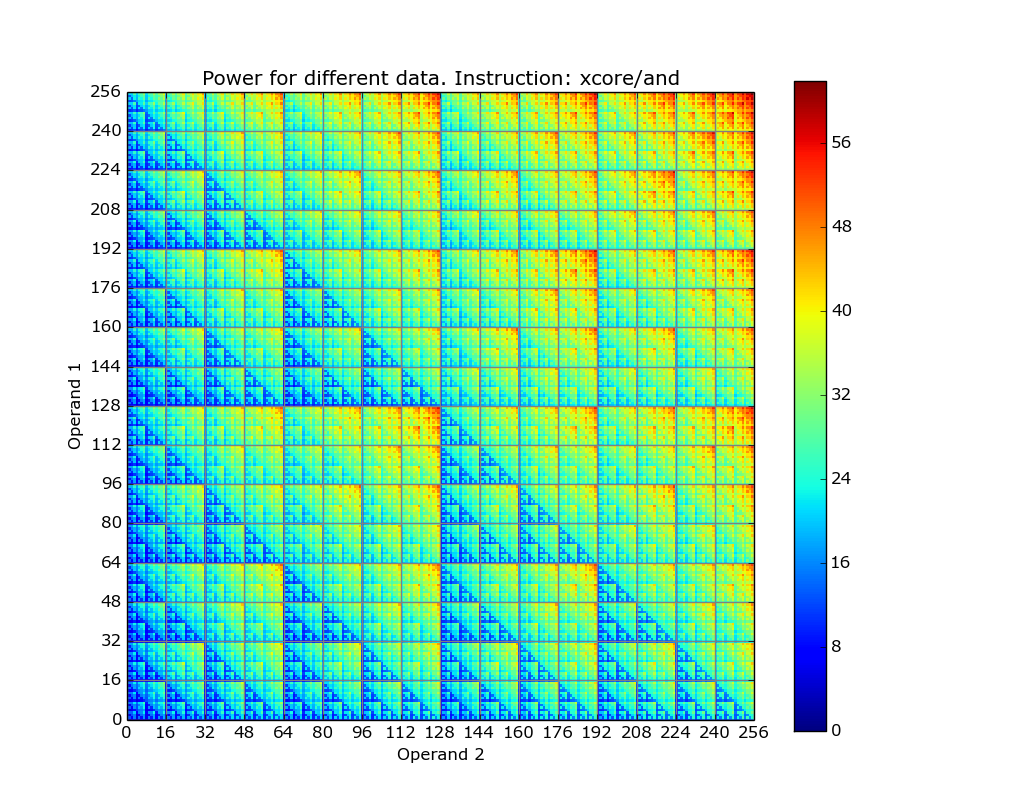
\includegraphics[width = 0.85\linewidth]{and_map}
    \caption{Dynamic power in milliwatts for XMOS XCore {\tt and} instruction.}
    \label{f:and-heatmap}
\end{figure}


- include the AND graph to illustrate different energy for different operands\todo{does and just take one cycle, so E=P?} 

- refer back to Tiwari 1994 where it was noted that measurements differed from predictions due to the fact that the actual operands of instructions are only known at runtime, so averages must be used for model characterization

- quote WCEC papers on data impact observed in practice [Jayanseelan WCEC]

- quote our work on WCEM and WCEM-theory

- single-value energy models: WC vs average

- need for tight but safe bounds

- statistic approaches need to be developed, i.e.\ characterize instructions in terms of energy consumption distributions [WCEM paper]



\subsection{Summary}

- pros and cons of energy modelling

- important characteristics of an energy model to support EE SWE

- need for timing and energy predictability

R.Wilhelm: Timing predictability of a hw/sw system is the degree to which bounds can be determined with acceptable precision, with acceptable effort and with acceptable loss of (average-case) performance. 
